\begin{titlepage} % Suppresses displaying the page number on the title page and the subsequent page counts as page 1
	\newcommand{\HRule}{\rule{\linewidth}{0.5mm}} % Defines a new command for horizontal lines, change thickness here
	
	\center % Centre everything on the page
	
	%------------------------------------------------
	%	Headings
	%------------------------------------------------
	
	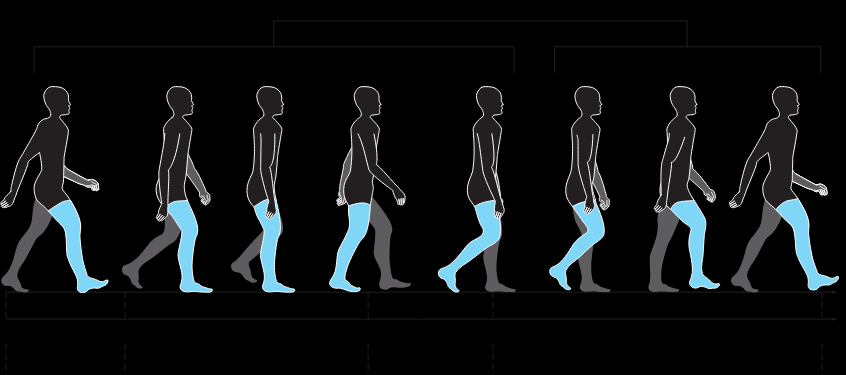
\includegraphics[width=0.75\textwidth]{Introwalking.png}

	%------------------------------------------------
	%	Title
	%------------------------------------------------
	
	\vspace{1.5cm}
	
	\HRule\\[0.6cm]
	
	{\huge\bfseries The ground reaction force of walking: a parameter to identify patients?} \\
	
	\vspace{1.0cm}
	
	{\large\bfseries Medical Data Science Project}\\[0.4cm] % Title of your document
	
	\HRule\\[1.5cm]
	
	%------------------------------------------------
	%	Author(s)
	%------------------------------------------------
	\large

	Name of the student:\\ 

	\huge

	Ursula \textsc{Trinler}

	%------------------------------------------------
	%	Date
	%------------------------------------------------
	
	\vfill\vfill % Position the date 3/4 down the remaining page
	
	{\large\today} % Date, change the \today to a set date if you want to be precise
	
	\vfill % Push the date up 1/4 of the remaining page
	
\end{titlepage}


%\end{document}